\section{Digital Waveform Generators (Chapter 8.1)}

%%%%%%%%%%%%%%%%%%%%%%%%%%%%%%%%%%%%%%%%%%%%%%%%%%%%%%%%%%%%
\subsection{Warum benötigt man digitale Wellenformgeneratoren?}

Ein DSP-System kann Signale nicht nur verarbeiten, sondern auch selbst erzeugen.

Typische Anwendungen sind:

\begin{itemize}
\item Musiksynthesizer
\item DTMF-Telefone
\item Testsignale
\item Radar- und Sonarsysteme
\item Modulationsverfahren
\end{itemize}

Ziel ist die Erzeugung eines gewünschten Signals mit möglichst geringem Rechenaufwand.

Grundsätzlich existieren zwei Methoden:

\begin{enumerate}
\item Rekursive Generatoren (filterbasiert)
\item Speicherbasierte Generatoren (Wavetable)
\end{enumerate}

\begin{center}
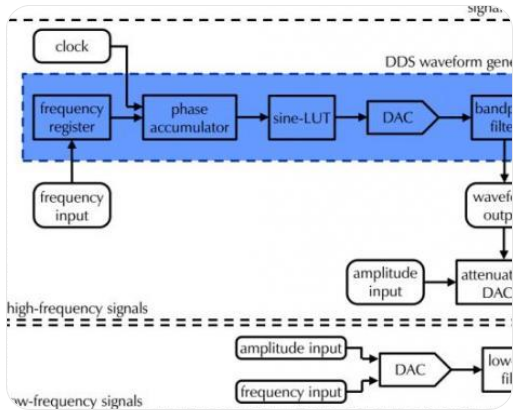
\includegraphics[width=0.8\linewidth]{images/generator_overview.png}
\end{center}

%%%%%%%%%%%%%%%%%%%%%%%%%%%%%%%%%%%%%%%%%%%%%%%%%%%%%%%%%%%%
\subsection{Grundidee digitaler Wellenformgeneratoren}

Ziel ist die Erzeugung einer gewünschten diskreten Wellenform $h(n)$.

Man entwirft ein System:

\[
H(z)
\]

dessen Impulsantwort genau der gewünschten Wellenform entspricht:

\[
h(n)
\]

Die gewünschte Wellenform kann erzeugt werden als:

\begin{enumerate}
\item Impulsantwort eines Filters
\item Wavetable mit gespeicherter Periode
\end{enumerate}

Ist das Signal periodisch, genügt es eine einzige Periode zu erzeugen und anschließend zyklisch zu wiederholen.

%%%%%%%%%%%%%%%%%%%%%%%%%%%%%%%%%%%%%%%%%%%%%%%%%%%%%%%%%%%%
\subsection{Zusammenhang zwischen Polen und Schwingungen}

Die wichtigste Erkenntnis dieses Kapitels lautet:

\begin{quote}
Jeder komplexe Pol erzeugt eine Schwingung.
\end{quote}

Ein Pol besitzt die Form

\[
p = Re^{j\omega_0}
\]

Dabei bestimmt

\begin{itemize}
\item der Radius $R$ die Dämpfung
\item der Winkel $\omega_0$ die Frequenz
\end{itemize}

\begin{center}
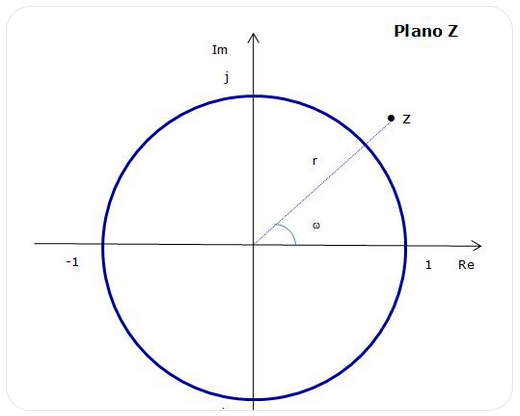
\includegraphics[width=0.5\linewidth]{images/pole_radius.png}
\end{center}

\begin{table}[h]
\centering
\begin{tabular}{c|c}
Radius & Wirkung \\
\hline
$R<1$ & gedämpfte Schwingung \\
$R=1$ & konstante Schwingung \\
$R>1$ & instabil \\
\end{tabular}
\end{table}

%%%%%%%%%%%%%%%%%%%%%%%%%%%%%%%%%%%%%%%%%%%%%%%%%%%%%%%%%%%%
\subsection{Sinusgenerator mittels Polstellen auf dem Einheitskreis}

\begin{center}
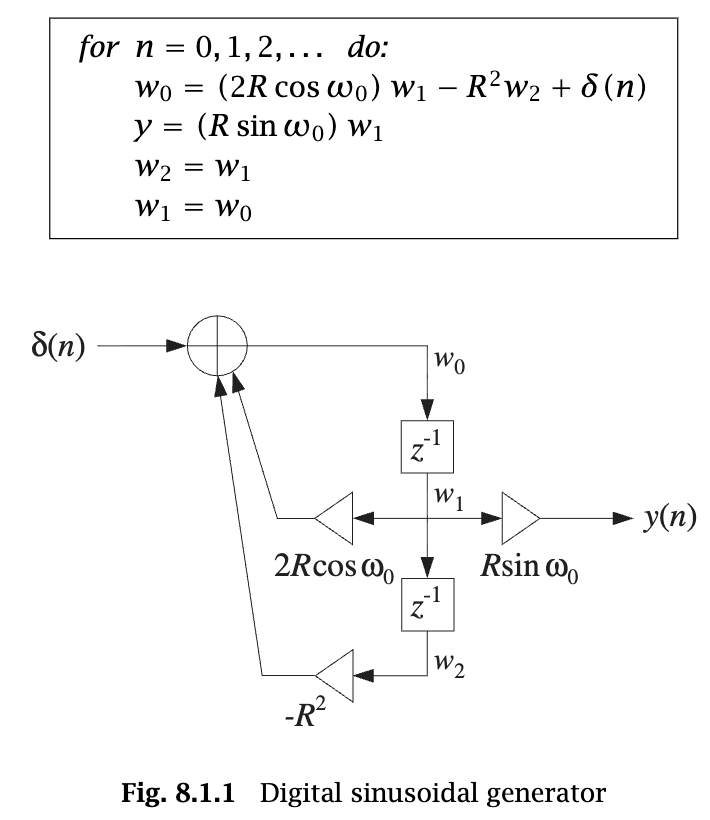
\includegraphics[width=0.8\linewidth]{images/sinusgenerator.png}
\end{center}

Die Pole liegen bei

\[
p_{1,2}=Re^{\pm j\omega_0}
\]

Die Übertragungsfunktion lautet:

\[
H(z)=
\frac{
R\sin(\omega_0)z^{-1}
}{
1-2R\cos(\omega_0)z^{-1}+R^2z^{-2}
}
\]

Impulsantwort:

\[
h(n)=R^n\sin(\omega_0 n)u(n)
\]

%%%%%%%%%%%%%%%%%%%%%%%%%%%%%%%%%%%%%%%%%%%%%%%%%%%%%%%%%%%%
\subsection{Warum entstehen Sinus und Kosinus?}

Grundlage ist die Euler-Formel:

\[
e^{j\omega n}
=
\cos(\omega n)
+
j\sin(\omega n)
\]

Konjugiert komplexe Pole erzeugen deshalb automatisch:

\[
R^n\cos(\omega n)
\]

und

\[
R^n\sin(\omega n)
\]

Deshalb basieren nahezu alle digitalen Oszillatoren auf komplex konjugierten Polen.

%%%%%%%%%%%%%%%%%%%%%%%%%%%%%%%%%%%%%%%%%%%%%%%%%%%%%%%%%%%%
\subsection{Kosinusgenerator}

\begin{center}
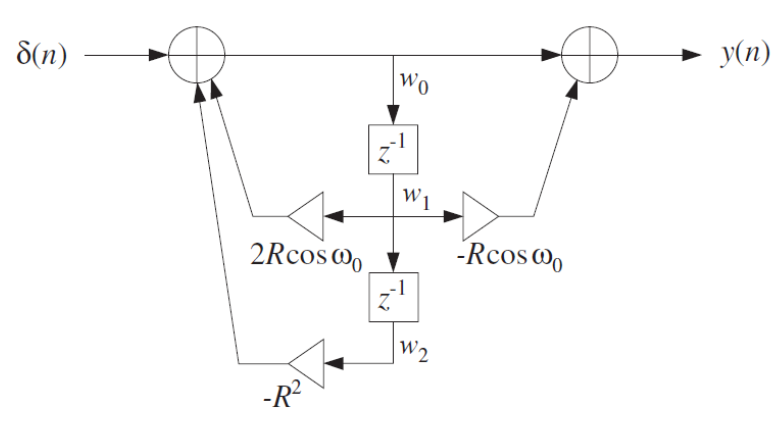
\includegraphics[width=0.8\linewidth]{images/cosinusgenerator.png}
\end{center}

\[
H(z)=
\frac{
1-R\cos(\omega_0)z^{-1}
}{
1-2R\cos(\omega_0)z^{-1}+R^2z^{-2}
}
\]

Impulsantwort:

\[
h(n)=R^n\cos(\omega_0n)u(n)
\]

%%%%%%%%%%%%%%%%%%%%%%%%%%%%%%%%%%%%%%%%%%%%%%%%%%%%%%%%%%%%
\subsection{Gekoppelte Realisierung (Coupled Form)}

\begin{center}
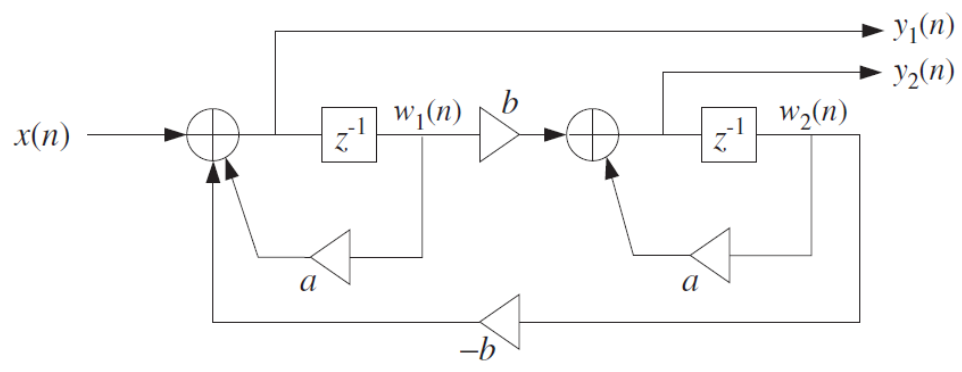
\includegraphics[width=0.8\linewidth]{images/coupledform.png}
\end{center}

Definiere:

\[
a=R\cos(\omega_0)
\]

\[
b=R\sin(\omega_0)
\]

Dann gilt:

\[
R^2=a^2+b^2
\]

Die Zustandsgrößen erfüllen:

\[
w_1(n) = a w_1(n-1) + b w_2(n-1)
\]

\[
w_2(n) = -b w_1(n-1) + a w_2(n-1)
\]

Diese Struktur erzeugt gleichzeitig Sinus und Kosinus.

%%%%%%%%%%%%%%%%%%%%%%%%%%%%%%%%%%%%%%%%%%%%%%%%%%%%%%%%%%%%
\subsection{Polstellenbetrachtung}

Für

\[
R=1
\]

liegen die Pole exakt auf dem Einheitskreis:

\[
p=e^{j\omega_0}
\]

\begin{center}
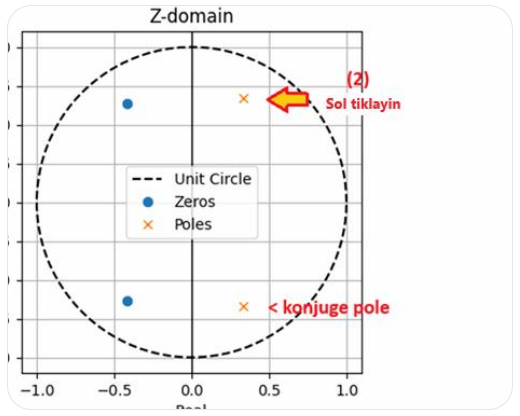
\includegraphics[width=0.5\linewidth]{images/unit_circle_poles.png}
\end{center}

Eigenschaften:

\begin{itemize}
\item Grenzstabil
\item Unendliche Sinusschwingung
\item Numerisch empfindlich
\end{itemize}

%%%%%%%%%%%%%%%%%%%%%%%%%%%%%%%%%%%%%%%%%%%%%%%%%%%%%%%%%%%%
\subsection{Periodische Wellenformgeneratoren}

Gegeben sei eine Periode mit Länge

\[
D
\]

Dann genügt die Spezifikation

\[
h(0),h(1),...,h(D-1)
\]

Die Grundfrequenz beträgt:

\[
f_0=\frac{f_s}{D}
\]

%%%%%%%%%%%%%%%%%%%%%%%%%%%%%%%%%%%%%%%%%%%%%%%%%%%%%%%%%%%%
\subsection{Filterbasierte Periodenerzeugung}

\begin{center}
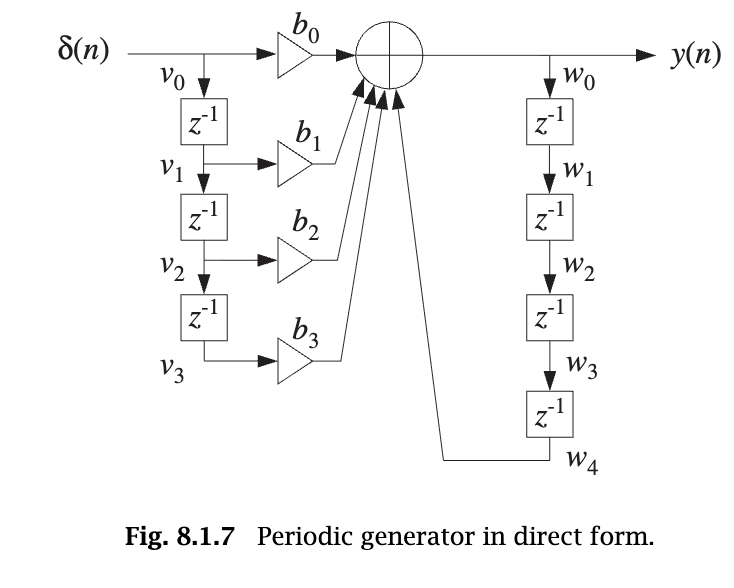
\includegraphics[width=0.8\linewidth]{images/periodic_generator.png}
\end{center}

Die zentrale Struktur lautet:

\[
H(z)= \frac{B(z)}{1-z^{-D}}
\]

Dabei gilt:

\[
\frac{1}{1-z^{-D}}= 1+z^{-D}+z^{-2D}+z^{-3D}+\dots
\]

Interpretation:

\begin{itemize}
\item Feedback erzeugt periodische Wiederholung
\item FIR-Teil formt die Periode
\end{itemize}

%%%%%%%%%%%%%%%%%%%%%%%%%%%%%%%%%%%%%%%%%%%%%%%%%%%%%%%%%%%%
\subsection{Polstellen periodischer Generatoren}

Die Pole ergeben sich aus:

\[
1-z^{-D}=0
\]

bzw.

\[
z^D=1
\]

Lösungen:

\[
z_k=e^{j2\pi k/D}
\]

\[
k=0,\dots,D-1
\]

\begin{center}
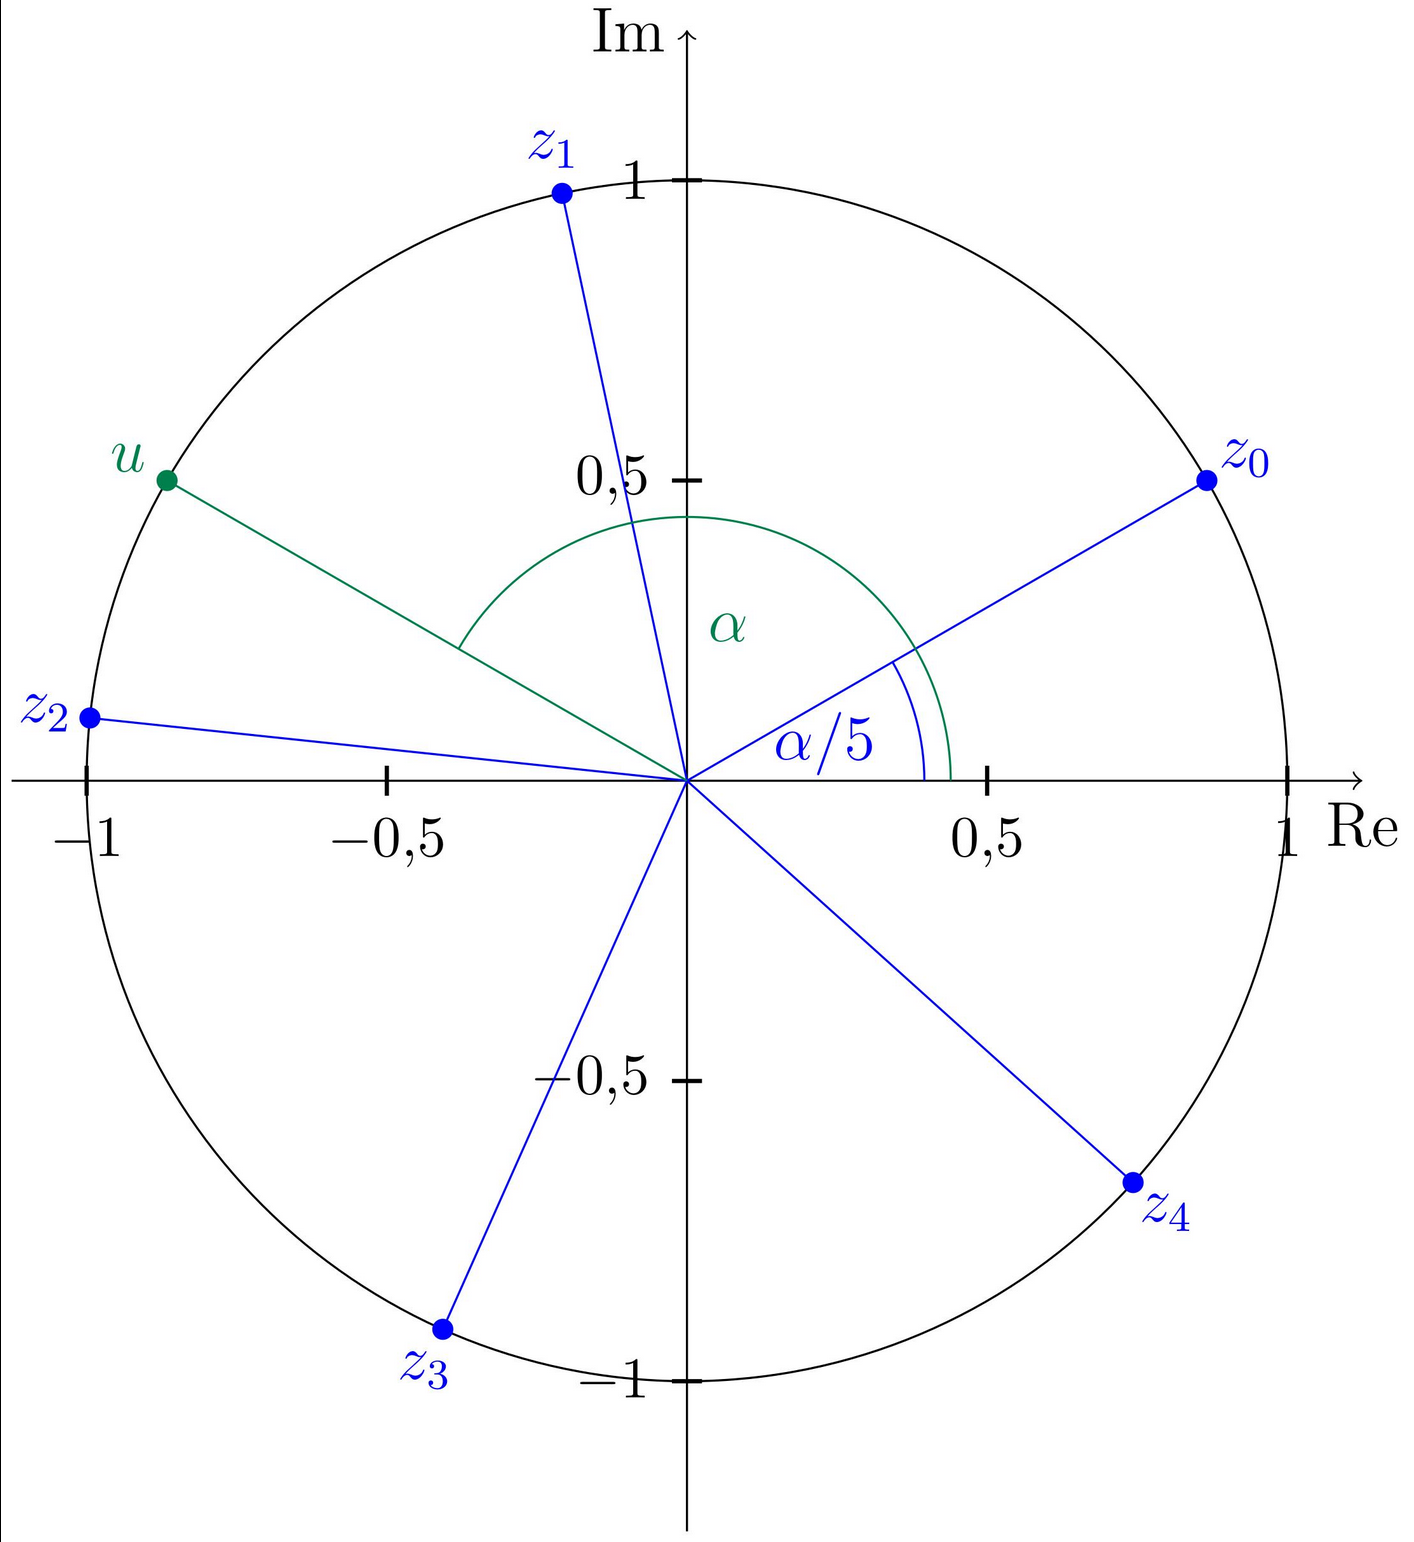
\includegraphics[width=0.5\linewidth]{images/dth_roots.png}
\end{center}

Alle Pole liegen auf dem Einheitskreis.

%%%%%%%%%%%%%%%%%%%%%%%%%%%%%%%%%%%%%%%%%%%%%%%%%%%%%%%%%%%%
\subsection{Direct Form und Canonical Form}

\begin{center}
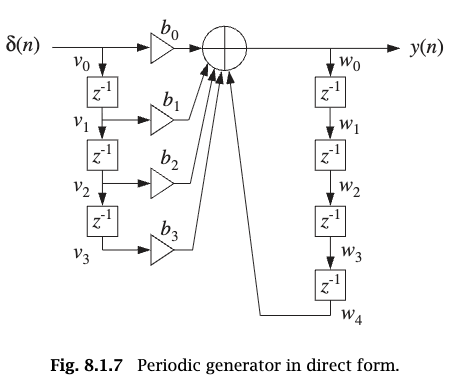
\includegraphics[width=0.8\linewidth]{images/direct_form.png}
\end{center}

\begin{center}
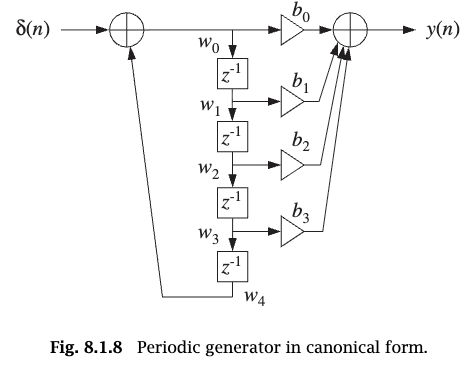
\includegraphics[width=0.8\linewidth]{images/canonical_form.png}
\end{center}

Direct Form:

\begin{itemize}
\item viele Delays
\item einfache Struktur
\end{itemize}

Canonical Form:

\begin{itemize}
\item minimale Anzahl Delays
\item speichereffizient
\item häufig in Aufgaben verwendet
\end{itemize}

%%%%%%%%%%%%%%%%%%%%%%%%%%%%%%%%%%%%%%%%%%%%%%%%%%%%%%%%%%%%
\subsection{Wavetable Generator}

Alternative zur Filterrealisierung:

Speichere eine Periode:

\[
w[0],w[1],...,w[D-1]
\]

Der Zeiger läuft zyklisch:

\[
y(n)=w[p(n)]
\]

\[
p(n+1) = (p(n)+c)\bmod D
\]

\begin{center}
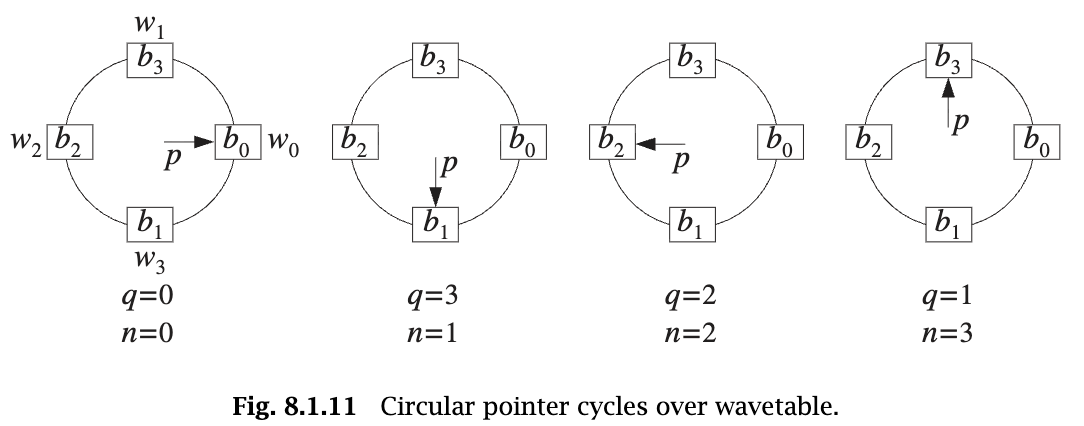
\includegraphics[width=0.7\linewidth]{images/wavetable_pointer.png}
\end{center}

Die Frequenz ergibt sich zu:

\[
f=c\frac{f_s}{D}
\]

%%%%%%%%%%%%%%%%%%%%%%%%%%%%%%%%%%%%%%%%%%%%%%%%%%%%%%%%%%%%
\subsection{Funktionsweise eines Wavetable-Generators}

Eine Periode wird einmal gespeichert.

Beispiel:

\[
[0,0.7,1,0.7,0,-0.7,-1,-0.7]
\]

Der Pointer bewegt sich durch die Tabelle:

\[
0 \rightarrow 1 \rightarrow 2 \rightarrow \dots
\]

Nach Erreichen des letzten Eintrags springt er zurück zum Anfang.

Dadurch entsteht ein periodisches Signal.

%%%%%%%%%%%%%%%%%%%%%%%%%%%%%%%%%%%%%%%%%%%%%%%%%%%%%%%%%%%%
\subsection{Interpolation bei nichtganzzahligen Indizes}

Für

\[
c=1.6
\]

entstehen Indizes:

\[
0, 1.6, 3.2, 4.8,\dots
\]

Diese liegen zwischen den gespeicherten Samples.

\begin{center}
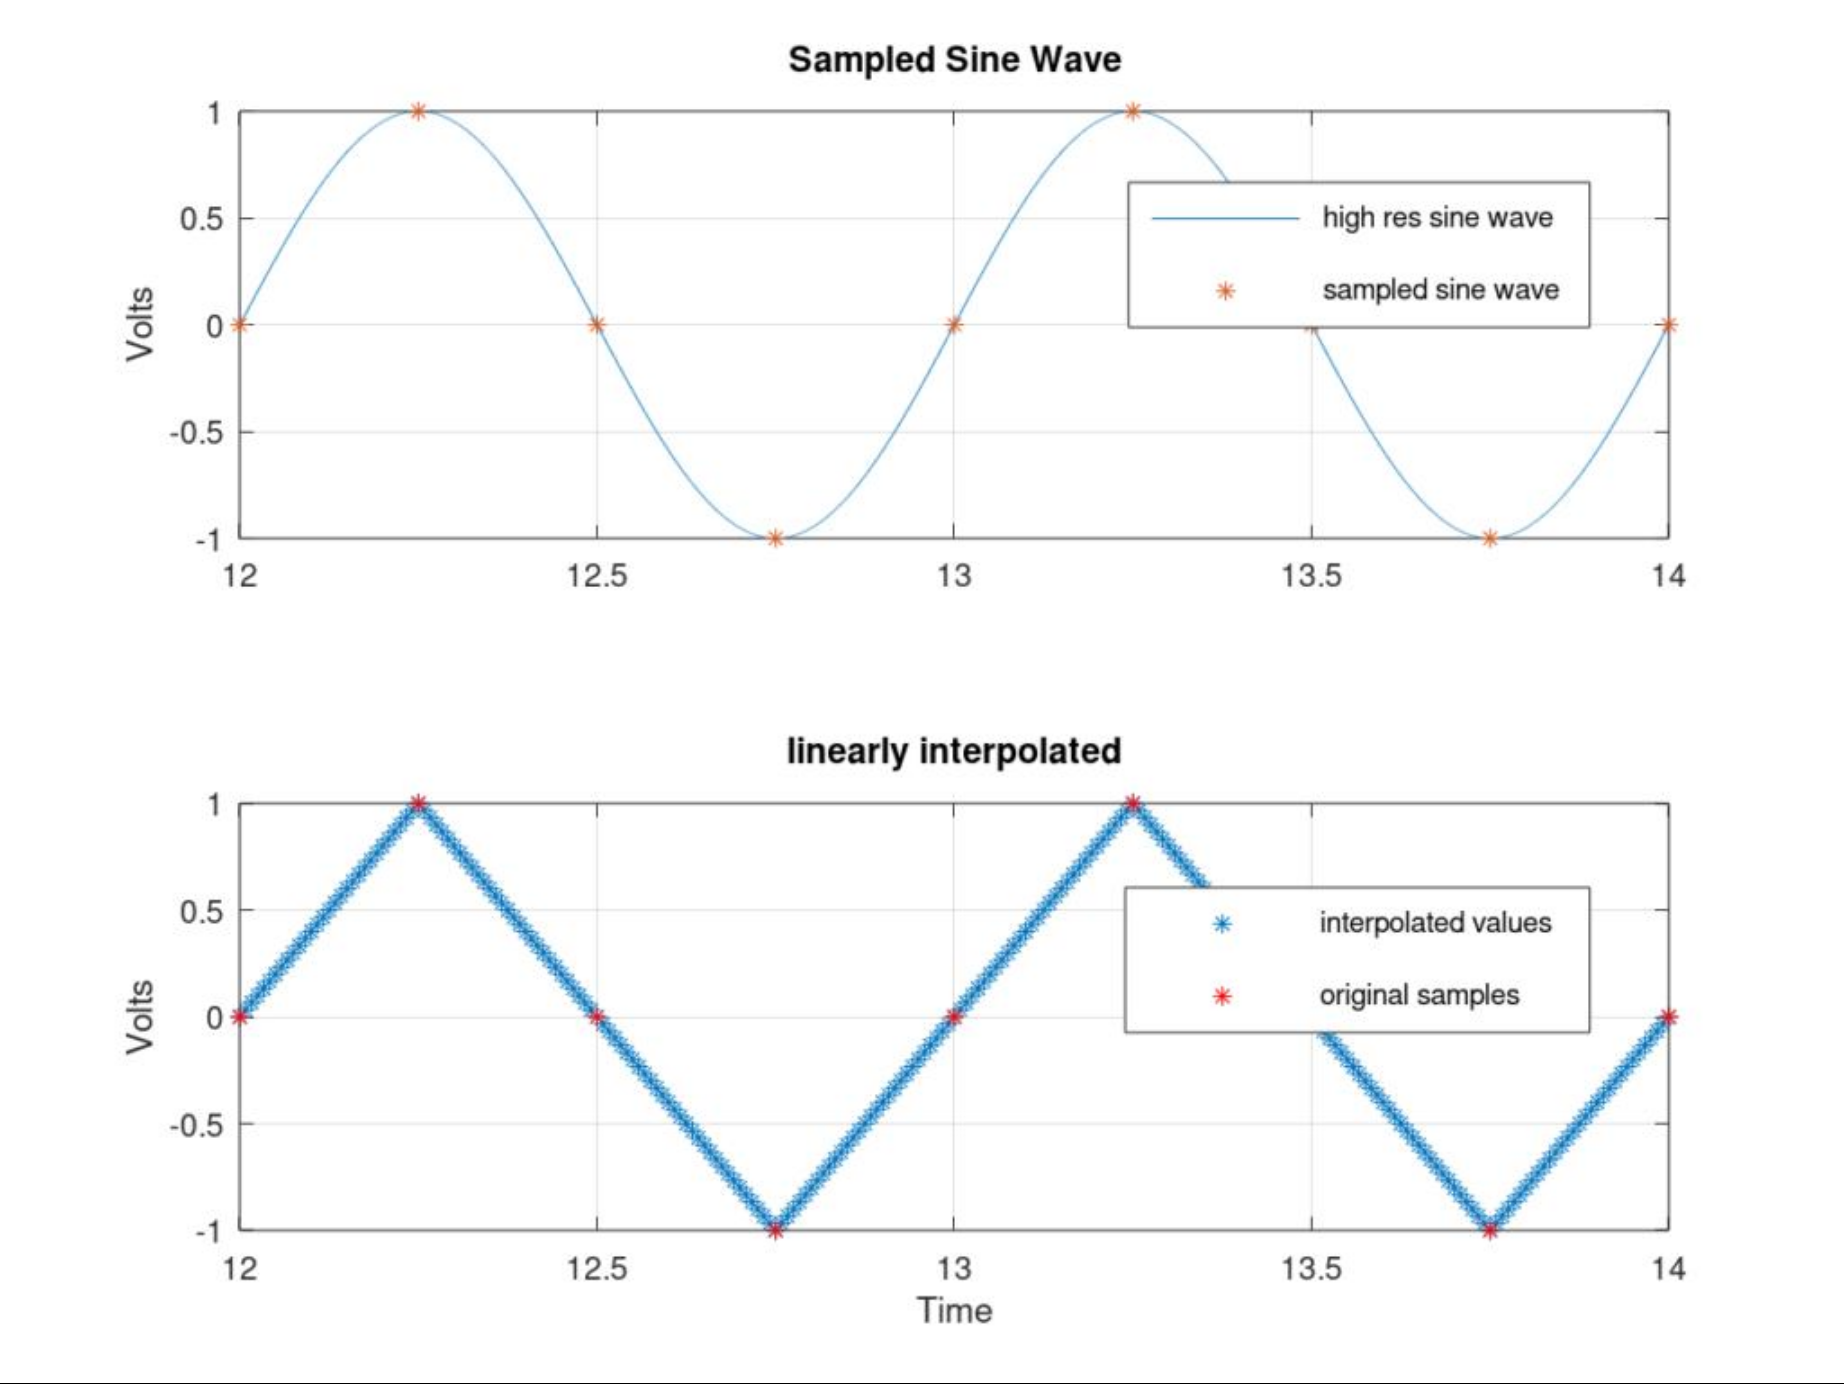
\includegraphics[width=0.6\linewidth]{images/interpolation.png}
\end{center}

Methoden:

\paragraph{Truncating Down}

\[
k=\lfloor i \rfloor
\]

\paragraph{Truncating Up}

\[
k=\lceil i \rceil
\]

\paragraph{Rounding}

\[
k=\text{round}(i)
\]

\paragraph{Lineare Interpolation}

\[
y=(1-\alpha)w[k]+\alpha w[k+1]
\]

%%%%%%%%%%%%%%%%%%%%%%%%%%%%%%%%%%%%%%%%%%%%%%%%%%%%%%%%%%%%
\subsection{Nyquist-Bedingung}

Für aliasfreie Erzeugung:

\[
\frac{-f_s}{2}<f<\frac{f_s}{2}
\]

Mit

\[
f=c\frac{f_s}{D}
\]

ergibt sich:

\[
-\frac{D}{2}<c<\frac{D}{2}
\]

%%%%%%%%%%%%%%%%%%%%%%%%%%%%%%%%%%%%%%%%%%%%%%%%%%%%%%%%%%%%
\subsection{Vergleich: Filtergenerator vs. Wavetable}

\begin{table}[h]
\centering
\begin{tabular}{c|c}
Filtergenerator & Wavetable \\
\hline
wenig Speicher & benötigt Speicher \\
Polanalyse möglich & sehr robust \\
theoretisch elegant & praktisch weit verbreitet \\
numerisch empfindlich & stabil \\
\end{tabular}
\end{table}

%%%%%%%%%%%%%%%%%%%%%%%%%%%%%%%%%%%%%%%%%%%%%%%%%%%%%%%%%%%%
\subsection{DTMF als Anwendung}

DTMF-Töne bestehen aus zwei Sinusfrequenzen:

\[
x(n)=\sin(\omega_1 n)+\sin(\omega_2 n)
\]

\begin{center}
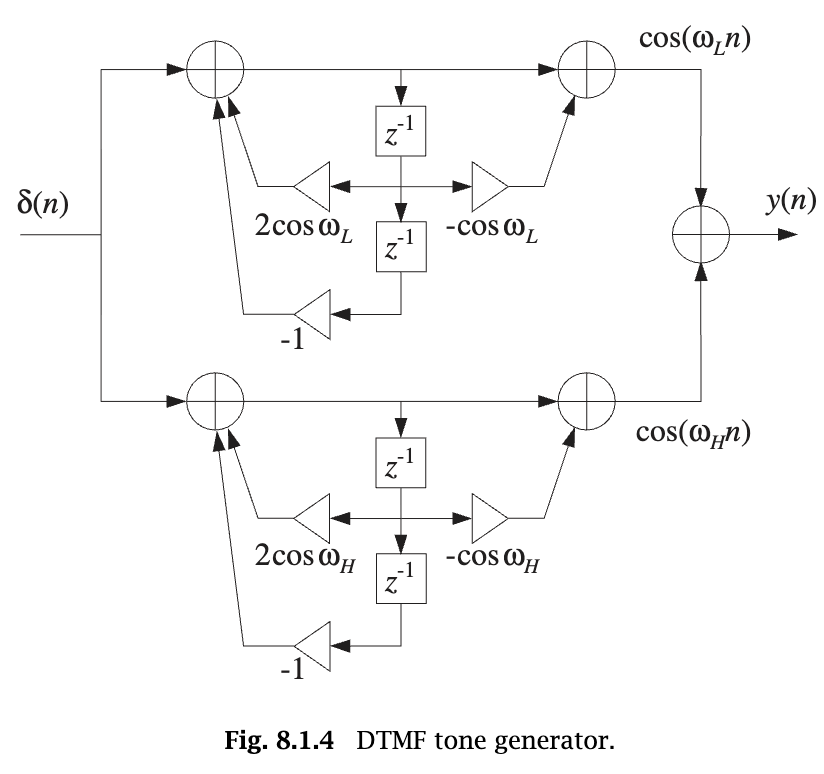
\includegraphics[width=0.8\linewidth]{images/dtmf_generator.png}
\end{center}

Realisierung:

\begin{itemize}
\item zwei Sinusgeneratoren
\item oder zwei Wavetable-Lookups
\end{itemize}

%%%%%%%%%%%%%%%%%%%%%%%%%%%%%%%%%%%%%%%%%%%%%%%%%%%%%%%%%%%%
\subsection{Zentrale Erkenntnisse}

\begin{itemize}
\item Komplexe Pole erzeugen Schwingungen.
\item Polwinkel bestimmt die Frequenz.
\item Polradius bestimmt die Dämpfung.
\item Periodische Generatoren basieren auf $1/(1-z^{-D})$.
\item Alle Pole periodischer Generatoren liegen auf dem Einheitskreis.
\item Wavetable-Generatoren speichern nur eine Periode.
\item Die Frequenz wird über die Schrittweite $c$ eingestellt.
\item Nichtganzzahlige Schrittweiten benötigen Interpolation.
\end{itemize}
